\documentclass[11pt]{article}
\usepackage[margin=1in]{geometry}

% Core packages
\usepackage{amsmath,amssymb}
\usepackage{tikz}
\usepackage{tikz-cd}
\usetikzlibrary{arrows.meta, positioning, shapes.geometric}
\usepackage{multicol}
\usepackage{hyperref}
\usepackage{booktabs}
\usepackage{array}
\usepackage{mathtools}

% Paragraphs
\setlength{\parindent}{0pt}
\setlength{\parskip}{0.8\baselineskip}

\title{\textbf{Signals and Systems}\\
\large A Review of Mathematical Modeling, State Machines, and Linear Systems}
\author{Shashwat Saxena\\IIIT Vadodara}
\date{June 2026}

\begin{document}
\maketitle
\tableofcontents
\newpage

 
\section{Introduction}

Signals are functions that map independent physical quantities (such as time or space) onto dependent physical quantities (such as air pressure or light intensity):
\[
  \text{signal}: \text{independentPhysicalQuantity} \rightarrow \text{dependentPhysicalQuantity}
\]

Systems are functions that transform or modify signals, mapping an input signal space onto an output signal space:
\[
  \text{system}: \text{inputSignalSpace} \rightarrow \text{outputSignalSpace}
\]

Together, signals and systems form the mathematical foundation of all communication, control, and signal processing theory.

 
\section{Signals}

\subsection{Continuous-Time and Discrete-Time Signals}

A \textbf{continuous-time signal} is defined for every value of time within an interval and is modeled as:
\[
  x : \mathbb{R} \rightarrow \mathbb{R}
\]
Examples include audio pressure waves, temperature profiles, and electrical voltages.

A \textbf{discrete-time signal} is defined only at specific instants, indexed by an integer $n$:
\[
  x : \mathbb{Z} \rightarrow \mathbb{R}
\]
Examples include sampled audio, digital images, and data sequences.

\subsection{Real-World Signal Models}

\subsubsection{Audio Signals}
An audio signal maps time onto the relative change in air pressure. Because sound is produced through compression and rarefaction of air, the time average of any audio signal is zero:
\[
  \text{audio} : \mathbb{R} \rightarrow \mathbb{R}, \quad \frac{1}{T}\int_0^T x(t)\,dt = 0
\]
Signals are normalised by subtracting the ambient (DC) pressure, leaving only the fluctuating component.

\subsubsection{Images}
A greyscale image maps a 2D spatial domain onto a scalar intensity:
\[
  \text{image}_\text{greyscale} : [0, H] \times [0, W] \rightarrow [0, B_{\max}]
\]
where $B_{\max}$ is the maximum brightness (white), and $0$ corresponds to black. In the mathematical vector-space formulation:
\[
  \text{image}_\text{greyscale} : \mathbb{R}^2 \rightarrow \mathbb{R}
\]
For a colour image, the co-domain becomes three-dimensional (red, green, blue channels):
\[
  \text{image}_\text{colour} : \mathbb{R}^2 \rightarrow \mathbb{R}^3
\]

\subsubsection{Video}
A video is a sequence of images (frames) displayed at a fixed frame rate. Formally, the $n^{\text{th}}$ frame is a function from spatial coordinates to intensity:
\[
  \text{video} : \mathbb{N} \rightarrow \left(\mathbb{R}^2 \rightarrow \mathbb{R}\right)
\]
The frame rate (frames per second) determines perceived smoothness.

\subsubsection{Sequences}
A sequence signal maps the natural numbers onto some entity:
\[
  \text{sequence} : \mathbb{N} \rightarrow \mathcal{E}
\]
Two common types are:
\begin{itemize}
  \item \textbf{Data sequences} — ordered records (e.g.\ stock prices, sensor logs).
  \item \textbf{Event streams} — timestamped occurrences (e.g.\ network packets, keyboard input).
\end{itemize}

 
\section{Systems}

A system $\mathcal{H}$ maps an input signal to an output signal:
\[
  \mathcal{H} : \text{inputSignalSpace} \rightarrow \text{outputSignalSpace}
\]

\subsection{Memoryless vs.\ Dynamic Systems}

A \textbf{memoryless} system's output depends only on the present input value:
\[
  y(t) = 2x(t)
\]

A \textbf{dynamic} system's output depends on past inputs or past outputs, requiring internal memory:
\[
  y(n) = x(n) + x(n-1)
\]

\subsection{Mathematical Models of Systems}

\subsubsection{Continuous-Time: Differential Equations}
Physical systems (RC circuits, thermal systems) are commonly described by ordinary differential equations. A general first-order system:
\[
  \frac{dy(t)}{dt} + ay(t) = bx(t)
\]

\subsubsection{Discrete-Time: Difference Equations}
Digital filters and sampled-data systems are described by difference equations. A first-order difference equation:
\[
  y(n+1) = ay(n) + bx(n)
\]

\subsection{System Composition}

Complex systems are built by composing simpler subsystems.

\subsubsection{Cascade (Series) Composition}
The output of $\mathcal{H}_1$ feeds into $\mathcal{H}_2$:
\[
  w(n) = \mathcal{H}_1\{x(n)\}, \qquad y(n) = \mathcal{H}_2\{w(n)\} = \mathcal{H}_2\{\mathcal{H}_1\{x(n)\}\}
\]
For LTI systems, cascade order is commutative: $\mathcal{H}_1 \circ \mathcal{H}_2 = \mathcal{H}_2 \circ \mathcal{H}_1$, and in terms of impulse responses:
\[
  h(n) = h_1(n) * h_2(n)
\]

\subsubsection{Parallel Composition}
Both systems receive the same input; outputs are summed:
\[
  y(n) = \mathcal{H}_1\{x(n)\} + \mathcal{H}_2\{x(n)\}
\]
For LTI systems, the equivalent impulse response is $h(n) = h_1(n) + h_2(n)$.

\subsubsection{Feedback Composition}
The output is routed back and subtracted from the input:
\[
  e(n) = r(n) - \mathcal{H}_2\{y(n)\}, \qquad y(n) = \mathcal{H}_1\{e(n)\}
\]
Solving for $y(n)$ gives the closed-loop transfer function:
\[
  y(n) = \frac{\mathcal{H}_1}{1 + \mathcal{H}_1 \mathcal{H}_2}\{r(n)\}
\]
Feedback introduces memory, enables self-regulation, and can stabilise otherwise unstable systems.

 
\section{Linear Time-Invariant (LTI) Systems}

\subsection{Linearity}

A system $\mathcal{H}$ is \textbf{linear} if it satisfies the superposition principle, which combines two properties:

\textbf{Homogeneity:} $\mathcal{H}\{ax\} = a\mathcal{H}\{x\}$

\textbf{Additivity:} $\mathcal{H}\{u + v\} = \mathcal{H}\{u\} + \mathcal{H}\{v\}$

Combined, for arbitrary scalars $a, b$:
\[
  \mathcal{H}\{au + bv\} = a\mathcal{H}\{u\} + b\mathcal{H}\{v\}
\]

\subsection{Time Invariance}

A system is \textbf{time-invariant} if its behaviour does not change with time. Equivalently, delaying the input by $n_0$ delays the output by the same amount:
\[
  x(n - n_0) \xrightarrow{\mathcal{H}} y(n - n_0)
\]

\subsection{SISO and MIMO Systems}

A \textbf{SISO} (Single-Input Single-Output) system has scalar input and output signals. Examples: an audio amplifier, an RC low-pass filter.

A \textbf{MIMO} (Multiple-Input Multiple-Output) system operates on vector-valued signals, commonly modelled as:
\[
  \mathbf{y}(t) = H\,\mathbf{x}(t), \quad H \in \mathbb{R}^{q \times m}
\]
Examples: multi-antenna wireless communication, aircraft control systems.

 
\section{State Spaces and State Machines}

\subsection{State Space}

The \textbf{state space} of a system is the minimum set of information required to completely determine all future outputs given any future input. For a Rubik's Cube, the state space is the set of all possible tile arrangements ($\approx 4.3 \times 10^{19}$ states).

\subsection{Finite State Machines (FSM)}

A Finite State Machine is formally a five-tuple:
\[
  \left(\mathcal{S},\, \mathcal{X},\, \mathcal{Y},\, f_{\text{update}},\, s_0\right)
\]
where $\mathcal{S}$ is the set of states, $\mathcal{X}$ the input alphabet, $\mathcal{Y}$ the output alphabet, $f_{\text{update}} : \mathcal{S} \times \mathcal{X} \rightarrow \mathcal{S}$ the transition function, and $s_0 \in \mathcal{S}$ the initial state.

A system is \textbf{deterministic} if $f_{\text{update}}$ maps each (state, input) pair to exactly one next state. It is \textbf{non-deterministic} if multiple next states are possible.

\subsection{Feedback and Fixed Points}

When a system's output feeds back into its input, steady-state behaviour is characterised by \textbf{fixed points}: values $x^*$ satisfying:
\[
  f(x^*) = x^*
\]

\textbf{Bisimulation} is a stronger notion of equivalence between two systems $A$ and $B$: both must simulate each other, meaning they are behaviourally indistinguishable from the outside.

 
\section{Linear State-Space Systems}

\subsection{The General Formulation}

For a discrete-time linear system, the state, input, and output are all vectors in real vector spaces:
\[
  \mathbf{s}(n) \in \mathbb{R}^p, \quad \mathbf{x}(n) \in \mathbb{R}^m, \quad \mathbf{y}(n) \in \mathbb{R}^q
\]

Since the system is linear, the update and output functions must be linear maps, represented by matrices. The \textbf{state-space equations} are:

\begin{align}
  \mathbf{s}(n+1) &= A\,\mathbf{s}(n) + B\,\mathbf{x}(n) \label{eq:state} \\
  \mathbf{y}(n)   &= C\,\mathbf{s}(n) + D\,\mathbf{x}(n) \label{eq:output}
\end{align}

The matrix dimensions must be consistent:

\begin{center}
\begin{tabular}{@{}lll@{}}
\toprule
Matrix & Dimension & Role \\
\midrule
$A$ & $p \times p$ & maps state to next state (system dynamics) \\
$B$ & $p \times m$ & maps input into the state \\
$C$ & $q \times p$ & maps state to output \\
$D$ & $q \times m$ & direct feedthrough from input to output \\
\bottomrule
\end{tabular}
\end{center}

\subsection{Solution to the State Equation}

For an autonomous system (no input, $\mathbf{x}(n) = \mathbf{0}$), equation~\eqref{eq:state} reduces to $\mathbf{s}(n+1) = A\,\mathbf{s}(n)$. Applying this recursively:
\[
  \mathbf{s}(n) = A^n\,\mathbf{s}(0)
\]
The long-term behaviour is entirely determined by the \textbf{eigenvalues} of $A$.

\subsection{Stability Analysis via Eigenvalues}

Let $\lambda_i$ denote the eigenvalues of $A$. For a scalar system ($p = 1$), $A$ is simply a scalar $a$, and $s(n) = a^n s(0)$. The stability conditions are:

\[
  |\lambda_i| < 1 \;\;\forall i \implies \text{asymptotically stable (response decays)}
\]
\[
  |\lambda_i| = 1 \;\;\forall i \implies \text{marginally stable (response constant amplitude)}
\]
\[
  \exists\, i : |\lambda_i| > 1 \implies \text{unstable (response grows without bound)}
\]

 
\section{Application I: The Discrete-Time Harmonic Oscillator}

\subsection{Motivation}

The goal is to construct a purely autonomous discrete-time system whose state traces a circle in $\mathbb{R}^2$ indefinitely — a \textbf{discrete-time harmonic oscillator}. The key insight is that repeated application of a 2D rotation matrix rotates a vector by the same angle at each step, tracing a circle.

\subsection{The Rotation Matrix}

A rotation by angle $\omega$ (radians) in $\mathbb{R}^2$ is represented by:
\[
  A = \begin{bmatrix} \cos\omega & -\sin\omega \\ \sin\omega & \cos\omega \end{bmatrix}
\]

Properties of $A$:
\begin{itemize}
  \item $\det(A) = \cos^2\omega + \sin^2\omega = 1$ — area-preserving.
  \item $A$ is orthogonal: $A^{-1} = A^\top$ — the inverse is just the transpose.
  \item Eigenvalues: $\lambda = e^{\pm j\omega}$, so $|\lambda| = 1$ — \textbf{marginally stable}.
\end{itemize}

Since all eigenvalues lie on the unit circle, the oscillation neither grows nor decays.

\subsection{State-Space Realization}

The state vector stores both coordinates of the rotating point:
\[
  \mathbf{s}(n) = \begin{bmatrix} s_1(n) \\ s_2(n) \end{bmatrix} = \begin{bmatrix} \cos(n\omega) \\ \sin(n\omega) \end{bmatrix}, \quad \mathbf{s}(0) = \begin{bmatrix} 1 \\ 0 \end{bmatrix}
\]

The state update equation expands to:
\[
  \begin{bmatrix} s_1(n+1) \\ s_2(n+1) \end{bmatrix}
  = \begin{bmatrix} \cos\omega & -\sin\omega \\ \sin\omega & \cos\omega \end{bmatrix}
  \begin{bmatrix} s_1(n) \\ s_2(n) \end{bmatrix}
\]
which gives the scalar recurrences:
\begin{align*}
  s_1(n+1) &= s_1(n)\cos\omega - s_2(n)\sin\omega \\
  s_2(n+1) &= s_1(n)\sin\omega + s_2(n)\cos\omega
\end{align*}

\subsection{Output}

Taking $C = \begin{bmatrix} 1 & 0 \end{bmatrix}$ extracts the first component:
\[
  y(n) = C\,\mathbf{s}(n) = s_1(n) = \cos(n\omega)
\]
The system output is a pure discrete-time cosine with no input required — all energy comes from the initial condition $\mathbf{s}(0)$.

\subsection{MATLAB Simulation}

In MATLAB, using $\omega = \pi/60$ rad/step and $n = 1000$ steps with $\mathbf{s}(0) = [0\;1]^\top$, the phase portrait (plot of $s_2$ vs.\ $s_1$) traces a perfect circle, confirming marginal stability.

 
\section{Application II: The 2-Tap Moving Average Low-Pass Filter}

\subsection{Motivation}

Consider a signal corrupted by high-frequency noise. The moving average filter recovers the underlying signal by averaging consecutive samples — high-frequency oscillations cancel, while the slowly-varying signal survives.

\subsection{The Difference Equation}

The 2-tap moving average is:
\[
  y(n) = \frac{x(n) + x(n-1)}{2}
\]
This is an \textbf{FIR} (Finite Impulse Response) filter: its output depends only on a finite window of past inputs, with no feedback from past outputs.

In the MATLAB model, the input signal is:
\[
  x(n) = \sin(2\pi \cdot 5 \cdot t_n) + 0.5\sin(2\pi \cdot 440 \cdot t_n), \quad F_s = 1000\,\text{Hz}
\]
a 5 Hz base signal corrupted by 440 Hz noise at half amplitude.

\subsection{State-Space Realization}

Choose the state $s(n) = x(n-1)$ (the one past sample required). Then $p = m = q = 1$, so all matrices reduce to scalars. The ABCD parameters are:

\[
  A = 0, \quad B = 1, \quad C = \tfrac{1}{2}, \quad D = \tfrac{1}{2}
\]

Substituting into equations~\eqref{eq:state}--\eqref{eq:output}:
\[
  s(n+1) = x(n) \qquad \text{(state stores current input)}
\]
\[
  y(n) = \tfrac{1}{2}x(n-1) + \tfrac{1}{2}x(n) \qquad \text{(output is the mean of current and previous input)}
\]

Interpretation of each parameter:
\begin{itemize}
  \item $A = 0$: the state does not feed back into itself — there are no autonomous dynamics.
  \item $B = 1$: the current input is stored directly into the state.
  \item $C = D = \tfrac{1}{2}$: the output is the average of the current and previous input.
\end{itemize}

Since $A = 0$, the zero-input response is $s(n) = 0^n \cdot s(0) = 0$ for all $n \geq 1$. The filter is unconditionally stable and entirely input-driven.

\subsection{Stability via Eigenvalues}

The single eigenvalue of $A$ is $\lambda = 0$, which satisfies $|\lambda| = 0 < 1$. The system is therefore \textbf{asymptotically stable} — in the absence of input, the state decays to zero in one step.

\subsection{Frequency Response}

To understand which frequencies the filter passes or rejects, apply a complex exponential input $x(n) = e^{j\omega n}$:
\[
  y(n) = \frac{1}{2}e^{j\omega n} + \frac{1}{2}e^{j\omega(n-1)} = e^{j\omega n} \cdot \frac{1}{2}\left(1 + e^{-j\omega}\right)
\]

The \textbf{frequency response} (eigenvalue of the LTI system for complex exponential input) is:
\[
  H(e^{j\omega}) = \frac{1}{2}\left(1 + e^{-j\omega}\right)
\]

Its magnitude is obtained by factoring out $e^{-j\omega/2}$:
\[
  \left|H(e^{j\omega})\right| = \left|\frac{e^{j\omega/2} + e^{-j\omega/2}}{2}\right| = \left|\cos\frac{\omega}{2}\right|
\]

This result directly explains the filter's behaviour:
\begin{itemize}
  \item $\omega = 0$ (DC): $|H| = |\cos 0| = 1$ — DC component passes through unchanged.
  \item $\omega = \pi$ (Nyquist frequency, highest possible): $|H| = |\cos(\pi/2)| = 0$ — completely rejected.
  \item The 440 Hz noise at $F_s = 1000$ Hz corresponds to normalized frequency $\omega = 2\pi \cdot 440/1000 = 0.88\pi$, which is near $\pi$ and thus strongly attenuated.
\end{itemize}

\subsection{Block Diagram}

\begin{center}
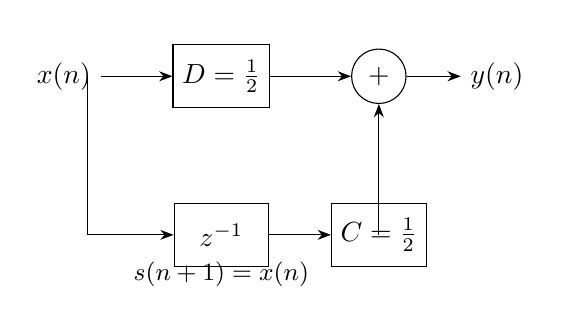
\begin{tikzpicture}[
  node distance=2cm,
  block/.style={draw, rectangle, minimum width=1.2cm, minimum height=0.8cm},
  sum/.style={draw, circle, minimum size=0.6cm},
  >=Stealth
]
  \node (in) {$x(n)$};
  \node[block, right of=in] (D) {$D = \frac{1}{2}$};
  \node[block, below=1.2cm of D] (delay) {$z^{-1}$};
  \node[block, right of=delay] (C) {$C = \frac{1}{2}$};
  \node[sum, right of=D] (plus) {$+$};
  \node[right of=plus, node distance=1.5cm] (out) {$y(n)$};

  \draw[->] (in) -- (D);
  \draw[->] (in) ++(0.3,0) |- (delay);
  \draw[->] (D) -- (plus);
  \draw[->] (delay) -- (C);
  \draw[->] (C) -| (plus);
  \draw[->] (plus) -- (out);
  \node[below of=delay, node distance=0.5cm] {\small $s(n+1) = x(n)$};
  \node[above of=in, node distance=0.5cm] {};
\end{tikzpicture}
\end{center}

There is no feedback path from output to input, confirming the FIR (no-IIR-poles) structure. The $z^{-1}$ block stores $x(n)$ and outputs $x(n-1)$ on the next step.

 
\section{Other MATLAB Models}

\subsection{Basic Discrete Signals}

The following elementary discrete-time signals were generated and plotted in MATLAB:

\begin{itemize}
  \item \textbf{Unit impulse:} $\delta(n) = \begin{cases} 1 & n = 0 \\ 0 & n \neq 0 \end{cases}$ — the fundamental building block of LTI analysis.
  \item \textbf{Unit step:} $u(n) = \begin{cases} 1 & n \geq 0 \\ 0 & n < 0 \end{cases}$
  \item \textbf{Unit ramp:} $r(n) = n\,u(n)$
  \item \textbf{Square pulse:} $p(n) = u(n) - u(n - N)$ for a pulse of width $N$.
  \item \textbf{Exponential decay:} $x(n) = a^n u(n)$, $|a| < 1$
\end{itemize}

Any discrete-time signal can be expressed as a weighted sum of shifted unit impulses:
\[
  x(n) = \sum_{k=-\infty}^{\infty} x(k)\,\delta(n - k)
\]
This decomposition is the basis of convolution and impulse response analysis.

\subsection{Amplitude Modulation (Communication Channel Simulator)}

A software AM modulator was built combining a 50 Hz baseband signal with a 220 Hz carrier wave. If the message signal is $m(t) = \cos(2\pi f_m t)$ and the carrier is $c(t) = \cos(2\pi f_c t)$, the AM signal is:
\[
  x_{\text{AM}}(t) = \left[1 + k_a m(t)\right] \cos(2\pi f_c t)
\]
where $k_a$ is the amplitude sensitivity. This model demonstrates signal preparation for transmission and visualises the modulation envelope in the time domain.

 
\section{Representation of Signals as Vector Spaces}

Every signal space can be given a vector-space structure. For instance, the set of square-integrable functions $L^2(\mathbb{R})$ forms a Hilbert space with inner product:
\[
  \langle x, y \rangle = \int_{-\infty}^{\infty} x(t)\,\overline{y(t)}\,dt
\]

This perspective unifies signal processing with linear algebra: filters are linear operators, frequency components are basis vectors (complex exponentials $\{e^{j\omega t}\}$), and the Fourier transform is a change of basis.

For the discrete-time signals studied in this work, the relevant space is $\ell^2(\mathbb{Z})$ — sequences with finite energy:
\[
  \|x\|^2 = \sum_{n=-\infty}^{\infty} |x(n)|^2 < \infty
\]

The frequency response $H(e^{j\omega})$ is the eigenvalue of an LTI system corresponding to the eigenfunction $e^{j\omega n}$, making eigenvalue analysis central to filter design.

\end{document}
